\pdfminorversion=4

~% if handout is on %~
    \documentclass[professionalfonts,handout]{beamer}
    \setbeameroption{show notes}
    \setbeamertemplate{note page}{\insertnote}
    \setbeamercolor{background canvas}{bg=white}
~% else %~
    ~% if interactive is on %~
        \documentclass[professionalfonts,handout]{beamer}
    ~% else %~
        \documentclass[professionalfonts]{beamer}
    ~% endif %~
~% endif %~



% Template original the Beamer: Copyright 2004 by Till Tantau <tantau@users.sourceforge.net>.


\mode<presentation>
{
  \usetheme{metropolis}
  % or ...

  %\setbeamercovered{transparent} %hace que lo que esta covered se muestre transparente
}

\setbeamertemplate{navigation symbols}{}%remove navigation symbols

\usepackage[english]{babel}

\usepackage[latin1]{inputenc}

\usepackage{times}
\usepackage[T1]{fontenc}

% para poder escribir codigo fuente en las diapositivas
\usepackage{listings}

% para graficar diagramas simples y arboles de jerarquias
\usepackage{tikz}
\usepackage{tikz-qtree}
\usetikzlibrary{matrix,positioning}
\usetikzlibrary{shapes,arrows,chains,calc,decorations.pathmorphing,decorations.shapes}

\definecolor{myLightGray}{RGB}{191,191,191}
\definecolor{myGray}{RGB}{160,160,160}
\definecolor{myDarkGray}{RGB}{144,144,144}
\definecolor{myDarkRed}{RGB}{167,114,115}
\definecolor{myRed}{RGB}{255,58,70}
\definecolor{myGreen}{RGB}{0,255,71}

\usepackage{xcolor}
\definecolor{darkgreen}{rgb}{0,.5,0}
\definecolor{darkblue}{rgb}{0,0,.7}
\lstdefinestyle{normal}{language=C++,       % lenguaje C++
   numbers=left,                            % enumerar las lineas
   keywordstyle=\color{darkblue}\textbf,    % color de las keywords
   stringstyle=\color{red},                 % color de los strings
   commentstyle=\color{darkgreen},          % color de los comentarios
   basicstyle=\color{black}\ttfamily\footnotesize\bfseries,     % color del texto en general
   morecomment=[l][\color{magenta}]{\#},    % coloreamos las intrucciones del precompilador (todo lo que empieza con #)
   ndkeywords={NULL,nullptr,siz,zer,mov,add,noexcept},               % definimos una nuevas keywords como NULL y nullptr
   ndkeywordstyle=\color{violet},           % y las nuevas keywords tendran este color
   frame=simple,                            % simple, sin ningun marco o frame alrededor del codigo
   basewidth={0.55em,0.55em}                % tamano de las letras/lineas. usado para reducir el whitespace entre estas
}

\lstdefinestyle{normal33}{language=C++,       % lenguaje C++
   numbers=left,                            % enumerar las lineas
   keywordstyle=\color{darkblue}\textbf,    % color de las keywords
   stringstyle=\color{red},                 % color de los strings
   commentstyle=\color{darkgreen},          % color de los comentarios
   basicstyle=\color{black}\ttfamily\footnotesize\bfseries,     % color del texto en general
   morecomment=[l][\color{magenta}]{\#},    % coloreamos las intrucciones del precompilador (todo lo que empieza con #)
   ndkeywords={NULL,nullptr},               % definimos una nuevas keywords como NULL y nullptr
   ndkeywordstyle=\color{violet},           % y las nuevas keywords tendran este color
   frame=simple,                            % simple, sin ningun marco o frame alrededor del codigo
   basewidth={0.55em,0.55em}                % tamano de las letras/lineas. usado para reducir el whitespace entre estas
}
%mismo estilo, sin numeros
\lstdefinestyle{normalnonumbers}{language=C++,
   keywordstyle=\color{darkblue}\textbf,
   stringstyle=\color{red},
   commentstyle=\color{darkgreen},
   basicstyle=\color{black}\ttfamily\footnotesize\bfseries,
   morecomment=[l][\color{magenta}]{\#},
   ndkeywords={NULL,nullptr,move,add},
   ndkeywordstyle=\color{violet},
   frame=simple,
   basewidth={0.55em,0.55em}
}


% mismo estilo pero todos los colores estan mas debiles como si se volvieran transparentes
% usado para poder resaltar el codigo.
\lstdefinestyle{dimmided}{language=C++,
   keywordstyle=\color{darkblue!30}\textbf,
   stringstyle=\color{red!30},
   commentstyle=\color{darkgreen!30},
   basicstyle=\color{black!30}\ttfamily\footnotesize\bfseries,
   morecomment=[l][\color{magenta!30}]{\#},
   ndkeywords={NULL,nullptr,siz,zer,mov,add},
   ndkeywordstyle=\color{violet!30},
   moredelim=**[is][\only<+->{\color{black}\lstset{style=normal}}]{@}{@}, % definimos que las lineas entre arrobas (@) tendran el estilo normal (con los colores a toda intensidad)
   frame=simple,
   basewidth={0.55em,0.55em}
}
\lstdefinestyle{dimmided42}{language=C++,
   keywordstyle=\color{darkblue!30}\textbf,
   stringstyle=\color{red!30},
   commentstyle=\color{darkgreen!30},
   basicstyle=\color{black!30}\ttfamily\footnotesize\bfseries,
   morecomment=[l][\color{magenta!30}]{\#},
   ndkeywords={NULL,nullptr,siz,zer,mov,add},
   ndkeywordstyle=\color{violet!30},
   moredelim=**[is][{\color{black}\lstset{style=normal}}]{@}{@}, % definimos que las lineas entre arrobas (@) tendran el estilo normal (con los colores a toda intensidad)
   frame=simple,
   basewidth={0.55em,0.55em}
}

\lstdefinelanguage{json}{
    literate=
     *{:}{{{\color{violet}{:}}}}{1}
      {,}{{{\color{violet}{,}}}}{1}
      {\{}{{{\color{darkgreen}{\{}}}}{1}
      {\}}{{{\color{darkgreen}{\}}}}}{1}
      {[}{{{\color{darkgreen}{[}}}}{1}
      {]}{{{\color{darkgreen}{]}}}}{1},
}


\lstdefinestyle{normaljson}{language=json,  % lenguaje json
   numbers=left,                            % enumerar las lineas
   keywordstyle=\color{darkblue}\textbf,    % color de las keywords
   stringstyle=\color{red},                 % color de los strings
   commentstyle=\color{red},                % color de los comentarios
   basicstyle=\color{black}\ttfamily\footnotesize\bfseries,     % color del texto en general
   morecomment=[l][\color{magenta}]{\#},    % coloreamos las intrucciones del precompilador (todo lo que empieza con #)
   ndkeywords={NULL,nullptr},               % definimos una nuevas keywords como NULL y nullptr
   ndkeywordstyle=\color{violet},           % y las nuevas keywords tendran este color
   frame=simple,                            % simple, sin ningun marco o frame alrededor del codigo
   basewidth={0.55em,0.55em}                % tamano de las letras/lineas. usado para reducir el whitespace entre estas
}

\lstdefinelanguage{http}{
    morekeywords={
        GET,
        PUT,
        POST,
        DELETE
    }
}

\lstdefinestyle{normalhttp}{language=http,  % lenguaje HTTP
   numbers=left,                            % enumerar las lineas
   keywordstyle=\color{darkblue}\textbf,    % color de las keywords
   stringstyle=\color{red},                 % color de los strings
   commentstyle=\color{red},                % color de los comentarios
   basicstyle=\color{black}\ttfamily\footnotesize\bfseries,     % color del texto en general
   morecomment=[l][\color{magenta}]{\#},    % coloreamos las intrucciones del precompilador (todo lo que empieza con #)
   ndkeywords={NULL,nullptr},               % definimos una nuevas keywords como NULL y nullptr
   ndkeywordstyle=\color{violet},           % y las nuevas keywords tendran este color
   frame=simple,                            % simple, sin ningun marco o frame alrededor del codigo
   basewidth={0.55em,0.55em}                % tamano de las letras/lineas. usado para reducir el whitespace entre estas
}

% Pone las constantes numericas con color (violeta en este caso):
% - los numeros que estan dentro de un string/comentarios NO son coloreados
% - los numeros por fuera que pertenecen a una palabra SON coloreados
%   (buf1, por ejemplo, el "1" es coloreado cuando no lo deberias. UPS!!)
% - No incluye el signo
%
%\lstset{literate=%
%  *{0}{{{\color{violet}0}}}1
%   {1}{{{\color{violet}1}}}1
%   {2}{{{\color{violet}2}}}1
%   {3}{{{\color{violet}3}}}1
%   {4}{{{\color{violet}4}}}1
%   {5}{{{\color{violet}5}}}1
%   {6}{{{\color{violet}6}}}1
%   {7}{{{\color{violet}7}}}1
%   {8}{{{\color{violet}8}}}1
%   {9}{{{\color{violet}9}}}1
%}

% Para resaltar lineas de codigo usando \btLstHLB{range} y \btLstHLB<overlay>{range}:
% Por ejemplo,
%  \btLstHLB{3}       linea 3 resaltada
%  \btLstHLB{1-5}     lineas de la 1 a la 5 resaltadas
%  \btLstHLB<2>{3}    linea 3 resaltada solo en el slide 2
%
% \btLstHLB usa un color azul mientras que \btLstHLR usa un color rojo como fondo
\usepackage{lstlinebgrd}
\makeatletter
\newcount\bt@rangea
\newcount\bt@rangeb

\newcommand\btIfInRange[2]{%
   \global\let\bt@inrange\@secondoftwo%
   \edef\bt@rangelist{#2}%
   \foreach \range in \bt@rangelist {%
      \afterassignment\bt@getrangeb%
      \bt@rangea=0\range\relax%
      \pgfmathtruncatemacro\result{ ( #1 >= \bt@rangea) && (#1 <= \bt@rangeb) }%
      \ifnum\result=1\relax%
      \breakforeach%
      \global\let\bt@inrange\@firstoftwo%
      \fi%
   }%
   \bt@inrange%
}
\newcommand\bt@getrangeb{%
   \@ifnextchar\relax%
   {\bt@rangeb=\bt@rangea}%
   {\@getrangeb}%
}
\def\@getrangeb-#1\relax{%
   \ifx\relax#1\relax%
      \bt@rangeb=100000%   \maxdimen is too large for pgfmath
   \else%
      \bt@rangeb=#1\relax%
   \fi%
}

%%%%%%%%%%%%%%%%%%%%%%%%%%%%%%%%%%%%%%%%%%%%%%%%%%%%%%%%%%%%%%%%%%%%%%%%%%%%%%
%
% \btLstHL<overlay spec>{range list}
%
\newcommand<>{\btLstHLB}[1]{%
   \only#2{\btIfInRange{\value{lstnumber}}{#1}{\color{blue!30}}% blue
   {\def\lst@linebgrdcmd####1####2####3{}}}%
}%
\newcommand<>{\btLstHLR}[1]{%
   \only#2{\btIfInRange{\value{lstnumber}}{#1}{\color{red!30}}% red
   {\def\lst@linebgrdcmd####1####2####3{}}}%
}%
%
%
%%%%%%%%%%%%%%%%%%%%%%

\makeatother


% sin fecha
\date{}

\author[7542-9508]{Di Paola Mart\'in \\ \texttt{martinp.dipaola <at> gmail.com} }

\institute[Universidad de Buenos Aires]
{
   Facultad de Ingenier\'ia\\
   Universidad de Buenos Aires
}

% Definimos una imagen para que este en cada slide
%\pgfdeclareimage[height=0.5cm]{university-logo}{imgs/fiuba.png}
%\logo{\pgfuseimage{university-logo}}

%% Definir estas en el documento final
%%
%% \title%
%% {Programaci\'on gen\'erica y templates en C++}
%%
%% \subject{Programaci\'on gen\'erica y templates en C++}


%%%%%
~% if interactive is on %~
    \AtBeginSection{}
    \AtBeginSubsection{}
~% else %~
    % At begin of each Section do nothing; at each Subsection show the Section and Subsection names
    % If the Section doesn't have a Subsection, then YOU must to add a unnumbered Subsection like \subsection*{}
    % so the AtBeginSubsection will get triggered
    \AtBeginSection{}
    \AtBeginSubsection[\frame{\subsectionpage}]{\frame{\subsectionpage}}
~% endif %~
%
%%%%%




\title%
{Manejo de Errores en C++}


\subject{Manejo de Errores en C++}


\begin{document}

\begin{frame}
   \titlepage
\end{frame}

\begin{frame}{De qu\'e va esto?}
   \tableofcontents
   % You might wish to add the option [pausesections]
\end{frame}


\section{Manejo de Errores}
\subsection{Motivaci\'on}
\begin{frame}[fragile]{El camino fel\'iz: mirada optimista pero ingenua}
   \begin{lstlisting}[style=normal]
void process() {
   char *buf = (char*) malloc(sizeof(char)*20);

   FILE *f = fopen("data.txt", "rt");

   fread(buf, sizeof(char), 20, f);

   /* ... */

   fclose(f);
   free(buf);
}
   \end{lstlisting}
\end{frame}
\note[itemize] {
\item C\'odigo simple pero sin chequeos. Un peligro!
\item Ignorar un error puede hacer que el programa crashee o se comporte de forma indefinida. Y lo que es peor, el crash se va a producir en un lugar distanciado de donde realmente hubo un error lo que lo hace mucho mas dif\'icil de debuggear.
}

\begin{frame}[fragile]{Contemplando el camino menos fel\'iz}
   \begin{lstlisting}[style=normal]
int process() {
   char *buf = (char*) malloc(sizeof(char)*20);

   FILE *f = fopen("data.txt", "rt");

   if(f == nullptr) {
      free(buf);
      return -1;
   }

   fread(buf, sizeof(char), 20, f);

   /* ... */
   fclose(f);
   free(buf);
}
   \end{lstlisting}
\end{frame}
\note[itemize] {
\item Para evitar que los errores pasen desapercibidos, hay que chequear y hay que hacerlo lo antes posible. Jam\'as se debe dejar que un error se propague ya que al final tendremos un programa err\'atico muy dif\'icil de debuggear.
\item Por cada chequeo hay que manualmente liberar los recursos anteriores.
\item Para que el caller sepa que sucedio, hay que retornar un c\'odigo de error.
}

\begin{frame}[fragile]{Mas robusto, pero poco fel\'iz: una mirada pesimista}
   \begin{lstlisting}[style=normal]
int process() {
   char *buf = (char*) malloc(sizeof(char)*20);
   if(buf == nullptr) { return -1; }

   FILE *f = fopen("data.txt", "rt");
   if(f == nullptr) { free(buf); return -2; } 

   int n = fread(buf, sizeof(char), 20, f);
   if(n < 0) { free(buf); fclose(f);  return -3; }

   /* ... */
   int s = fclose(f);
   if(s != 0) { free(buf); return -4; }

   free(buf);
}
   \end{lstlisting}
\end{frame}
\note[itemize] {
\item Al final, tantos chequeos hacen engorrozo un c\'odigo que era sencillo
\item En C se usan otras estrategias. En C++ se usan Excepciones
}

\subsection{Excepciones y su Mal Uso}
\begin{frame}[fragile]{Las excepciones no implican un buen manejo de errores}
   \begin{lstlisting}[style=normal,linebackgroundcolor={%
         \only<1>{\def\lst@linebgrdcmd####1####2####3{}}%
         \btLstHLB<2>{4,7,10,13}%
         \btLstHLB<3>{14}%
         \btLstHLB<4>{3-10,15-17}%
         \btLstHLB<5>{3-7,15-17}%
   }]
void process() {
   try {
      char *buf = (char*) malloc(sizeof(char)*20);
      if(buf == nullptr) { throw -1; }

      FILE *f = fopen("data.txt", "rt");
      if(f == nullptr) { throw -2; } 

      int n = fread(buf, sizeof(char), 20, f);
      if(n < 0) { throw -3; }

      int s = fclose(f);
      if(s != 0) { throw -4; }
   } catch(...) {
      free(buf);
      fclose(f);
      throw;  // re lanza la excepcion
   }
   \end{lstlisting}
\end{frame}
\note[itemize] {
\item Lanzamos una excepci\'on con la instrucci\'on \lstinline[style=normal]!throw!
\item En un primer approach, las excepciones nos evitan tener que retornar c\'odigos de error
\item Usando \lstinline[style=normal]!try-catch! atrapamos las excepciones para centralizar la liberaci\'on de los recursos
\item Una vez hecho esto, la instrucci\'on \lstinline[style=normal]!throw! dentro de un \lstinline[style=normal]!catch! relanza la excepcion atrapada asi quien nos llam\'o (el caller de la funci\'on \lstinline[style=normal]!process!) sabe que algo sali\'o mal.
\item \alert{Y el c\'odigo queda cada vez peor!!} Este es un ejemplo de un \alert{mal manejo de los errores}: el uso de excepciones no garantiza un buen manejo de los errores.
\item El c\'odigo es tan complejo que estoy liberando un recurso sin antes haberlo adquirido y encima tengo un leak!!
}


\subsection{RAII: Excepciones Bien Usadas}
\begin{frame}[fragile]{RAII: Resource Acquisition Is Initialization}
   \begin{lstlisting}[style=normal]
class Buffer{
   char *buf;

   public:
   Buffer(size_t count) : buf(nullptr) {
      buf = (char*) malloc(sizeof(char)*count);
      if (!buf) { throw -1; }
   }

   /* ... */

   ~Buffer() {
      free(buf); //No pregunto si es nullptr o no!
   }
};
   \end{lstlisting}
\end{frame}
\note[itemize] {
\item Todo recurso debe ser encapsulado en una clase
\item El constructor se encarga de adquirirlo y el destructor de liberarlo
\item Si durante la construcci\'on del objeto algo sale mal, lanzar un excepci\'on.
\item Aplicable a Sockets, Buffers, Files, Mutexs, Locks, etc...
}

\begin{frame}[fragile]{RAII y la vuelta al camino fel\'iz}
   \begin{lstlisting}[style=normal,linebackgroundcolor={%
         \only<1>{\def\lst@linebgrdcmd####1####2####3{}}%
         \btLstHLB<2>{2-6,11}% 
         \btLstHLB<3>{2-4,11}% 
   }]
void process() {
   Buffer buf(20);

   File f("data.txt", "rt");

   f.read(buf->raw_ptr(), sizeof(char), 20);

   /* ... */

   f.close();
} // Destruyo los objetos creados
   \end{lstlisting}
\end{frame}
\note[itemize] {
\item C\'odigo simple pero con chequeos ocultos en cada objeto RAII
\item Si hay un error, se lanza una excepci\'on. Los errores no se silencian. Se hacen todos los chequeos en un solo lugar: la clase que encapsula al recurso.
\item Al salir del scope, por proceso normal o por excepci\'on, los objetos construidos son destruidos mientras que los objetos que no fueron construidos no se destruyen: no hay leaks ni tampoco \lstinline[style=normal]!free!(s) de objetos sin alocar.
\item Es importante resaltar esto: los objetos RAII deben adquirir los recursos en sus constructores y destruirlos en sus destructores y cada objeto RAII debe hacerse cargo del recurso que encapsula, si algo sale mal, lanzar una excepci\'on.
}

\begin{frame}[fragile]{Si el constructor falla, el destructor no se invoca.}
   \begin{lstlisting}[style=normal]
class DoubleBuffer {
   char *bufA;
   char *bufB;
   /* ... */

   DoubleBuffer(size_t count) : bufA(nullptr), bufB(nullptr) {
      bufA = (char*) malloc(sizeof(char)*count);
      bufB = (char*) malloc(sizeof(char)*count);
      
      if(!bufA || !bufB) throw -1; // Leak!
   }

   ~DoubleBuffer() {
      free(bufA);
      free(bufB);
   }
   \end{lstlisting}
\end{frame}
\note[itemize] {
\item El destructor se llama sobre objetos bien construidos. Si hay una excepci\'on en el constructor de \lstinline[style=normal]!DoubleBuffer!, C++ va a considerar que el objeto no fue construido y por ende no debe destruirse asi que no se le llamara a su destructor. Es importante escribir los constructores con sumo cuidado.
\item Para evitar problemas, revisar dos veces la implementaci\'on de los constructores
}

\begin{frame}[fragile]{RAII over RAII}{}
   \begin{lstlisting}[style=normal]
class DoubleBuffer {
   Buffer bufA;   // No son punteros, ese es el truco!
   Buffer bufB;
   /* ... */

   DoubleBuffer(size_t count) : bufA(count), bufB(count) {
   }  //Constructor simple, sin try-catch

   ~DoubleBuffer() {
   }
   \end{lstlisting}
\end{frame}
\note[itemize] {
\item Al usar objetos RAII como atributos de otros objetos (y no punteros a...), los destructores se llaman autom\'aticamente sobre los objetos creados
\item Si el primer \lstinline[style=normal]!Buffer! (\lstinline[style=normal]!bufA!) se creo pero el segundo fall\'o, solo el destructor de \lstinline[style=normal]!bufA! se va a llamar.
}

\begin{frame}[fragile]{RAII - Ejemplos}
   \begin{lstlisting}[style=normal]
class Socket {
   public:
      Socket(/*...*/) {
         this->fd = socket(AF_INET, SOCK_STREAM, 0);
         if (this->fd == -1) 
            throw OSError("The socket cannot be created.");
      }

      ~Socket() {
         close(this->fd);
      }
};
   \end{lstlisting}
\end{frame}

%TODO estaria bueno hacer que un codigo se muestre solo despues de otro:
\begin{frame}[fragile]{RAII - Ejemplos}
   \begin{lstlisting}[style=normal]
class Lock {
   Mutex &mutex;

   public:
      Lock(Mutex &mutex) : mutex(mutex) {
         mutex.lock();
      }

      ~Lock() {
         mutex.unlock();
      }
   \end{lstlisting}
   \begin{columns}
      \begin{column}{.5\linewidth}
         \begin{lstlisting}[style=normal]
void change_shared_data() {
   this->mutex.lock();
   /* ... */
   this->mutex.unlock();
}
         \end{lstlisting}
      \end{column}
      \begin{column}{.4\linewidth}
         \begin{lstlisting}[style=normal]
void change_shared_data() {
   Lock lock(this->mutex);
   /* ... */

}
         \end{lstlisting}
      \end{column}
   \end{columns}
\end{frame}

\begin{frame}[fragile]{RAII - Resumen}
   \begin{itemize}
      \item Los recursos deben ser encapsulados en objetos, adquiriendolos en el constructor y liberandolos en el destructor.
      \item Hacer uso del stack. Los objetos del stack son siempre destruidos al final del scope llamando a su destructor.
      \item Los objetos que encapsulan recursos deben detectar condiciones an\'omalas y lanzar una excepci\'on.
      \item Pero \alert{jam\'as} lanzar una excepci\'on en un destructor. (Condici\'on \lstinline[style=normal]!noexcept!)
      \item Una excepci\'on en un constructor hace que el objeto no se cree (y su destructor no se llamara). Liberar sus recursos \alert{a mano} antes de salir del constructor.
      \item Cuidado con copiar objetos RAII. En general es mejor hacerlos no-copiables y movibles.
   \end{itemize}
\end{frame}


\section{Exception Safety}
\begin{frame}[fragile]{No s\'olo es una cuesti\'on de leaks}
   \begin{lstlisting}[style=normal]
struct Date {
   void set_day(int day) {
      this._day = day;   if (/* invalid */) throw -1;
   }

   void set_month(int month) {
      this._month = month;  if (/* invalid */) throw -1;
   }
}
try {
   Date d(30, 04);
   d.set_day(31);
   d.set_month(01);
} catch(...) {
   std::cout << d;
}
   \end{lstlisting}
El estado final del objeto \lstinline[style=normal]!d! es \dots
\pause
\lstinline[style=normal]!31/04!, no tiene sentido!!
\end{frame}
\note[itemize] {
\item Los errores pueden suceder en cualquier momento. No solo hay que evitar leaks (y otros) sino que tambi\'en hay que tratar de dejar a los objetos en un estado consistente y sin corromper (donde siguen manteniendo sus invariantes).
\item Claramente la estrategia "modifico el objeto y luego chequeo" no trae mas que problemas.
}

\begin{frame}[fragile]{Exception safe weak (o basic): objetos consistentes.}
   \begin{lstlisting}[style=normal]
struct Date {
   void set_day(int day) {
      if (/* invalid */) throw -1;  this._day = day;  
   }

   void set_month(int month) {
      if (/* invalid */) throw -1;  this._month = month; 
   }
}
try {
   Date d(30, 01);
   d.set_day(31);
   d.set_month(02);
} catch(...) {
   std::cout << d;
}
   \end{lstlisting}
Y ahora?
\pause
imprime \lstinline[style=normal]!31/01!, fecha v\'alida pero no es la original.
\end{frame}
\note[itemize] {
\item Con una simple modifici\'on de c\'odigo se puede mejorar mucho la situaci\'on.
\item Ante un error el objeto no queda corrupto (sigue manteniendo sus invariante) aunque puede no quedar en un estado definido.
\item Cuando ante una excepci\'on un objeto no se corrompe pero no queda en el estado anterior se dice que el m\'etodo en cuesti\'on es exception safe weak.
}

\begin{frame}[fragile]{Exception safe strong: objetos inalterados.}
   \begin{lstlisting}[style=normal]
struct Date {
   void load_date(int day, int month) {
      if (/* invalid */) throw -1;
      this.set_day(day);
      this.set_month(month);
   }

   void set_day(int day) { /* ... */ }
   void set_month(int month) { /* ... */ }
}
try {
   Date d(28, 01);
   d.load_date(31, 02);
} catch(...) {
   std::cout << d;
}
   \end{lstlisting}
Ahora imprime \lstinline[style=normal]!28/01!, el objeto \alert{no cambi\'o}.
\end{frame}
\note[itemize] {
\item Cuando ante una excepci\'on un objeto no se corrompe y adem\'as queda en el estado anterior se dice que el m\'etodo en cuesti\'on es exception safe strong.
\item Los objetos deber\'ian en lo posible implementar sus m\'etodos como exception safe strong. No siempre es posible, pero en la medida que se pueda deber\'ia intentarse.
}

\begin{frame}[fragile]{Encapsulaci\'on de objetos y Exception safety}
Los setters son un peligro, no es posible garantizar una interfaz strong exception safe:
   \begin{lstlisting}[style=normal]
   public:
      void load_date(int day, int month);
      void set_day(int day);
      void set_month(int month);
   \end{lstlisting}
Pero si la interfaz esta bien dise\~nada, es m\'as f\'acil hacer garant\'ias:
   \begin{lstlisting}[style=normal]
   public:
      void load_date(int day, int month);

   private:
      void set_day(int day);
      void set_month(int month);
   \end{lstlisting}
\end{frame}
\note[itemize] {
\item El manejo de errores y las excepciones no se pueden agregar al final de un proyecto, deben dise\~narse en conjunto con el resto del objeto pues para poder garantizar los exception safe weak/strong y se requiere de un dise\~no cuidadoso de la interfaz.
\item A grandes razgos, los m\'etodos set son los causantes de muchos problemas por que pueden dejar inv\'alidos a los objetos, sobre todo si algo falla en el medio. Evitar a toda costa los set.
\item La encapsulaci\'on de un objeto no significa "poner los atributos privados y los getters y setters p\'ublicos" sino que significa "poner todo privado salvo los m\'etodos que no pueden dejar inconsistente al objeto".
\item Por ejemplo, sea la fecha \lstinline[style=normal]!Date d(30, 04)! y se quiere cambiar a \lstinline[style=normal]!28/02! (ambas fechas v\'alidas). Usando solamente los m\'etodos \lstinline[style=normal]!set_day! y \lstinline[style=normal]!set_month!, en que orden hay que invocar a esos m\'etodos para obtener la fecha requerida? F\'acil no? Y si ahora de la fecha \lstinline[style=normal]!30/04! se quiere ir a \lstinline[style=normal]!31/01!? Vale el mismo orden o lo tuviste que cambiar? \lstinline[style=normal]!:)! Los setters son malos.
}

\begin{frame}[fragile,plain]{El dise\~no de la interfaz es afectada}
   \begin{lstlisting}[style=normal,linebackgroundcolor={%
         \only<1>{\def\lst@linebgrdcmd####1####2####3{}}%
         \btLstHLB<2>{7}%
         \btLstHLB<3>{8}% 
         \btLstHLB<4>{10}%
         \only<5>{\def\lst@linebgrdcmd####1####2####3{}}%
         \btLstHLR<6>{9}% 
   }]
template<class T>
T Stack::pop() {
   if (count_elements == 0) {
      throw "Stack empty";
   }
   else {
      T temp;
      temp = elements[count_elements-1];
      --count_elements;
      return temp;
   }
}
   \end{lstlisting}
    \vspace{-0.5cm}
\only<1-4>{
Qu\'e puede salir mal y lanzar una excepci\'on?
   \begin{itemize}
      \item<2-> El constructor por default.
      \item<3-> El operador asignaci\'on (=).
      \item<4-> El constructor por copia.
   \end{itemize}
}
\only<5>{
Hay posibilidad de leak? Es exception safe weak o strong?
}
\only<6->{El constructor por copia nos arruina. No hay forma de poner un \lstinline[style=normal]!try!-\lstinline[style=normal]!catch! y revertir "\lstinline[style=normal]!--count_elements!".\\
   Por eso los containers del est\'andar ofrecen dos m\'etodos, \lstinline[style=normal]!void pop()! y \lstinline[style=normal]!T top()!.
}
\end{frame}
\note[itemize] {
\item Los containers de C++ son exception safe strong.
\item Este ejemplo explica por que el \lstinline[style=normal]!std::stack! de C++ tiene un \lstinline[style=normal]!void pop()! a diferencia de otros lenguages donde el \lstinline[style=normal]!pop()! retorna el objeto sacado.
}

\begin{frame}[fragile]{Exception Safety - Resumen}
   \begin{itemize}
      \item Tratar de dejar los objetos inalterados (Exception safe strong)
      \item No poner setters. Es muy f\'acil equivocarse y dejer objetos inconsistentes.
   \end{itemize}
\end{frame}


\section{Excepciones, y ahora qu\'e?}
\begin{frame}[fragile]{Recolectar la mayor informaci\'on posible}
   \visible<2>{Pobre}
   \begin{lstlisting}[style=normal]
void parser(/* ... */) {
   /* ... */
   if (/* error */) 
      throw ParserError();
   /* ... */
}
   \end{lstlisting}

   \visible<2>{Mucho mejor}
   \begin{visibleenv}<2>
   \begin{lstlisting}[style=normal, breaklines=true]
void parser(/* ... */) {
   /* ... */
   if (/* error */) 
      throw ParserError("Encontre %s pero esperaba %s en el archivo %s, linea %i", found, expected, filename, line);
   /* ... */
}
   \end{lstlisting}
\end{visibleenv}
\end{frame}
\note[itemize] {
\item Lo m\'as importante es explicar el error. No usar decenas de clases de errores, solo usar una o dos y que estas reciban un mensaje como par\'ametro
\item Los mensajes deben ser lo mas descriptivos posibles. Piensen en ustedes mismos tratando de entender un error, no seria mejor que el mensaje de la excepci\'on les diga qu\'e paso y en d\'onde? Hasta ser\'ia mejor si les dice las posibles causas y soluciones!
\item No hacer \lstinline[style=normal]!throw new Error()! (usa el heap), usar directamente \lstinline[style=normal]!throw Error()!. Eviten usar el heap innecesariamente.
}


\begin{frame}[fragile]{Una excepci\'on por dentro}
   \begin{lstlisting}[style=normal]
#include <typeinfo>

#define BUF_LEN  256

class OSError : public std::exception {
   private:
   char msg_error[BUF_LEN];

   public:
   explicit OSError(const char* fmt, ...) noexcept;
   virtual const char *what() const noexcept;
   virtual ~OSError() noexcept {}
};
   \end{lstlisting}
\end{frame}
\note[itemize] {
\item En C++ cualquier cosa puede ser una excepci\'on: un \lstinline[style=normal]!int!, un puntero, un objeto. Pero es preferible un objeto cuya clase herede de \lstinline[style=normal]!std::exception!.\\
\item Implementar un m\'etodo \lstinline[style=normal]!what()! para retornar el mensaje de error.
\item Los m\'etodos con la keyword \lstinline[style=normal]!noexcept! en sus firmas dicen "este m\'etodo no lanzar\'a ninguna excepci\'on". Si el m\'etodo no cumple su promesa, todo el programa crashea (se invoca a la funci\'on \lstinline[style=normal]!terminate!).
\item En C++ se puede decir que excepciones un m\'etodo puede llegar a lanzar escribiendo en su firma por ejemplo \lstinline[style=normal]!int metodo() throw(OutOfRange)! pero eviten usar este feature como documentaci\'on sobre que excepci\'ones se podr\'ian lanzar o no (al estilo Java). Hace que sus clases sean \alert{mas dif\'iciles} de extender.
}

\begin{frame}[fragile]{Wrappeo de errores de C y del sistema operativo}
   \begin{lstlisting}[style=normal,linebackgroundcolor={%
         \btLstHLB<1>{5}%
         \btLstHLB<2>{4,7-10}%
         \btLstHLB<3>{5,12,13}% 
   }]
#include <errno.h>
#include <cstdio>
#include <cstdarg>
OSError::OSError(const char* fmt, ...) noexcept {
    _errno = errno;

    va_list args;
    va_start(args, fmt);
    int s = vsnprintf(msg_error, BUF_LEN, fmt, args);
    va_end(args);

    strncpy(msg_error+s, strerror(_errno), BUF_LEN-s);
    msg_error[BUF_LEN-1] = 0;
}
   \end{lstlisting}
   \begin{itemize}
      \only<1> {
      \item Copiar \lstinline[style=normal]!errno! antes de hacer cualquier cosa.
      }
      \only<2> {
      \item Obtener un mensaje explicativo del contexto. Aceptar un mensaje de error y argumentos variables como lo hace \lstinline[style=normal]!printf!. 
      }
      \only<3> {
      \item Obtener un mensaje del sistema operativo con \lstinline[style=normal]!strerror!. Cuidado que no es \alert{not thread safe}, usar \lstinline[style=normal]!strerror_r!.\\
      }
   \end{itemize}
\end{frame}
\note[itemize] {
\item Muchas funciones del sistema operativo y de C en general dicen "retorna -1 en caso de error". Esas funciones guardan en la variable global \lstinline[style=normal]!errno! un c\'odigo de error m\'as descriptivo que un simple \lstinline[style=normal]!-1!
\item Como \lstinline[style=normal]!errno! es una variable global cualquier funci\'on puede modificarla. Ante la detecci\'on de un error, se debe copiar \lstinline[style=normal]!errno! \alert{inmediatamente} para tener una copia del c\'odigo sin miedo a que otra funci\'on posterior la sobreescriba
\item El valor de \lstinline[style=normal]!errno! puede ser traducido a un mensaje de error con \lstinline[style=normal]!strerror! o \lstinline[style=normal]!strerror_r!, este \'ultimo thread safe.
\item Muchas funciones de socket optan por otro mecanismo y hay que usar \lstinline[style=normal]!gai_strerror!
\item Tanto C como C++ pueden definir funciones con una lista variable de argumentos (variadic). \lstinline[style=normal]!printf! es un ejemplo.
\item En general es muy conveniente que las excepciones soporten un constructor que acepte un formato y un n\'umero variable de argumentos como \lstinline[style=normal]!printf! guardandose el mensaje formateado.
}

\begin{frame}[fragile]{Clases de excepciones como discriminantes}
   \begin{columns}
      \begin{column}{.5\linewidth}
         \begin{lstlisting}[style=normal]
try {
   parser();
} catch(const CharNotFound &e) {
   printf("%s", e.what());
} catch(const ExprInvalid &e) {
   printf("%s", e.what());
} catch(const SyntacticError &e) {
   printf("%s", e.what());
} catch(const ParserError &e) {
   printf("%s", e.what());
} catch(const std::exception &e) {
   printf("%s", e.what());
} catch(...) { // ellipsis: catch anything
   printf("Unknow error!");
}
         \end{lstlisting}
      \end{column}
      \begin{column}{.4\linewidth}
         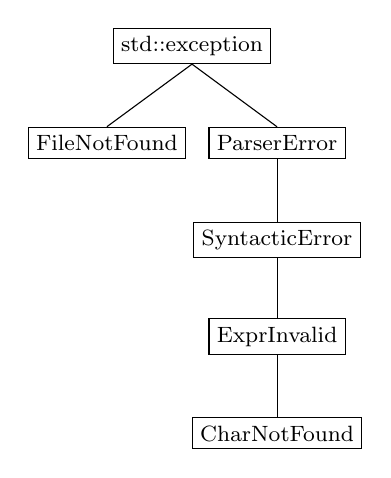
\begin{tikzpicture}[every tree node/.style=draw]\footnotesize
            \tikzset{level distance=35pt}
            \Tree [.{std::exception}
                     [.{FileNotFound} ]
                     [.{ParserError}
                        [.{SyntacticError}
                           [.{ExprInvalid}
                               {CharNotFound}
                           ]
                        ]
                     ]
                  ]
            \end{tikzpicture}
      \end{column}
   \end{columns}
\end{frame}
\note[itemize] {
\item Los \lstinline[style=normal]!catch! funcionan de forma polim\'orfica. La clase de una excepci\'on no necesariamente debe coincidir con la firma del \lstinline[style=normal]!catch!: un \lstinline[style=normal]!catch! m\'as gen\'erico puede atrapar la excepci\'on igualmente.
\item De esto se deduce que los \lstinline[style=normal]!catch! mas gen\'ericos deben estar al final
\item Si una excepci\'on no es atrapada, continua su viaje por el stack
\item Preferir la expresi\'on \lstinline[style=normal]!const Exception&! para atrapar excepciones. Al usar referencias se evitan copias.
}

\begin{frame}[fragile]{Simplificar!}
   \begin{columns}
      \begin{column}{.5\linewidth}
         \begin{lstlisting}[style=normal]
try {
   parser();
} catch(const std:exception &e) {
   printf("%s", e.what());
} catch(...) {
   printf("Unknow error!");
}
         \end{lstlisting}
      \end{column}
      \begin{column}{.4\linewidth}
         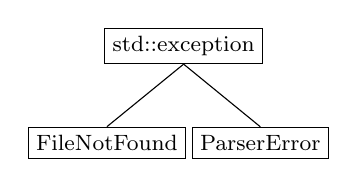
\begin{tikzpicture}[every tree node/.style=draw]\footnotesize
            \tikzset{level distance=35pt}
            \Tree [.{std::exception}
                     [.{FileNotFound} ]
                     [.{ParserError}  ]
                  ]
            \end{tikzpicture}
      \end{column}
   \end{columns}
    \begin{itemize}
        \item Pocas clases de errores: no necesitamos tanto poder de discriminaci\'on. Menos clases y mejor hechas con buenos mensajes de error.
        \item Pocos \lstinline[style=normal]!catch!, solo poner aquellos que van a hacer algo distinto con la excepci\'on.
    \end{itemize}
\end{frame}
\note[itemize] {
\item Como las clases de excepciones se usan principalmente como discriminantes en los \lstinline[style=normal]!catch!, la raz\'on de tener varias clases es por que hay c\'odigos distintos a ejecutar en cada \lstinline[style=normal]!catch!.
\item En la pr\'actica el c\'odigo que se encuentra en los \lstinline[style=normal]!catch! es de simple loggueo que aplica a todos los errores en general. Por lo tanto no deber\'ian haber muchas clases de errores sino unas pocas pero con buenos mensajes de error.
}

\begin{frame}[fragile]{Basta de prints! Loguear a un archivo con syslog}
   \begin{lstlisting}[style=normal, breaklines=true]
   syslog(LOG_DEBUG, "Mensaje de debug.");
   
   syslog(LOG_INFO, "Un mensaje informativo:"
                    "escuchando en el puerto %i", port);
   
   syslog(LOG_CRIT, "Un error: %s", e.what());
   \end{lstlisting}
\end{frame}
\note[itemize] {
\item En vez de logguear a la consola con un \lstinline[style=normal]!printf! se puede logguear a traves de una librer\'ia llamada \lstinline[style=normal]!syslog! (para linux) que logguea directamente a un archivo (t\'ipicamente\lstinline[style=normal]!/var/log/messages! o \lstinline[style=normal]!/var/log/syslog!) 
\item \lstinline[style=normal]!syslog! permite logguear poniendo data extra en los mensajes: el process id, el timestamp. Data muy \'util si se trabaja con m\'ultiples procesos.
\item Hay otras libs \'utiles similares a \lstinline[style=normal]!syslog! como \lstinline[style=normal]!log4j! o \lstinline[style=normal]!log4cpp! entre otras, todas con las mismas capacidades.
\item Vean la p\'agina de manual de \lstinline[style=normal]!syslog!.
}

\begin{frame}[fragile]{No dejar escapar a ninguna excepci\'on}
   \begin{lstlisting}[style=normal, breaklines=true]
int main(int argc, char *argv[]) try {
   /* ... */
   return 0;

} catch(const std::exception &e) {
   syslog(LOG_CRIT, "[Crit] Error!: %s", e.what());
   return 1;

} catch(...) {
   syslog(LOG_CRIT, "[Crit] Unknow error!");
   return 1;
}
   \end{lstlisting}
\end{frame}
\note[itemize] {
\item Nunca dejar escapar una excepci\'on. En C++ causan un crash.
\item En todo el c\'odigo deber\'ian haber apenas unos pocos \lstinline[style=normal]!try-catch!. Uno de los lugares en donde deber\'ian estar es en el \lstinline[style=normal]!main! para atrapar y logguear cualquier excepci\'on antes de que escape del \lstinline[style=normal]!main! y hagan crashear el programa.
}

% Solo quiero 3 secciones, \section*{Resumen}
\begin{frame}[fragile]{Resumen}
   \beamerdefaultoverlayspecification{<+->}
   \begin{itemize}
      \item RAII + Objetos en el Stack == (casi) \alert{ning\'un leak} y no hay necesidad de \lstinline[style=normal]!try/catch! para liberar recursos. Mantener a los objetos consistentes.
      \item RAII + Buena Interfaz == Chequeos (al estilo pesimista) en un \alert{solo lugar} (no hay que repetirlos). Quien use esos objetos puede asumir que todo va a salir bien (mirada optimista).
      \item Chequeos + Excepciones con info + Loggueo a un archivo (Los errores no se silencian, sino que se detectan, propagan y registran) == El debuggeo es \alert{m\'as f\'acil}.
      \item Clases de Errores: Usar las que tiene el est\'andar C++. Crear las propias pero s\'olo si hacen falta.
      \item \lstinline[style=normal]!try/catch!: Deber\'ian haber pocos. En el \lstinline[style=normal]!main! y tal vez en alg\'un constructor en particular.
   \end{itemize}
\end{frame}

\appendix
\section<presentation>*{\appendixname}
\subsection<presentation>*{Referencias}

\begin{frame}[allowframebreaks]
   \frametitle<presentation>{Referencias}

   \begin{thebibliography}{10}

         \beamertemplatebookbibitems
         % Start with overview books.

      \bibitem{Sutter}
         Herb Sutter.
         \newblock {\em Exceptional C++: 47 Engineering Puzzles}.
         \newblock Addison Wesley, 1999.

      \bibitem{Stroustrup}
         Bjarne Stroustrup.
         \newblock {\em The C++ Programming Language}.
         \newblock Addison Wesley, Fourth Edition.

         \beamertemplatearticlebibitems
         
      \bibitem{man page: syslog}
         man page: syslog
         
         % Followed by interesting articles. Keep the list short. 

   \end{thebibliography}
\end{frame}

\end{document}


